\documentclass{article}
% Change "article" to "report" to get rid of page number on title page
\usepackage{amsmath,amsfonts,amsthm,amssymb}
\usepackage{setspace}
\usepackage{upgreek}
\usepackage{Tabbing}
\usepackage{fancyhdr}
\usepackage[utf8]{inputenc}

\usepackage{lastpage}
\usepackage{extramarks}
\usepackage{chngpage}
\usepackage{soul,color}
\usepackage{sagetex}
\usepackage{tikz}
\usetikzlibrary{arrows,automata}
\usetikzlibrary{shapes.arrows,chains,positioning}
\usepackage{fancybox}
\usepackage{graphicx,float,wrapfig}

% In case you need to adjust margins:
\topmargin=-0.45in      %
\evensidemargin=0in     %
\oddsidemargin=0in      %
\textwidth=6.5in        %
\textheight=9.0in       %
\headsep=0.25in         %

% Homework Specific Information
\newcommand{\hmwkTitle}{Tarea \#2}
\newcommand{\hmwkDueDate}{Lunes,\ Febrero\ 15,\ 2010}
\newcommand{\hmwkClass}{CC3006}
\newcommand{\hmwkClassTime}{}
\newcommand{\hmwkClassInstructor}{Bidkar Pojoy}
\newcommand{\hmwkAuthorName}{Carlos E. L\'{o}pez Camey}


\newcommand{\set}[1]{\{ #1  \}}


% Setup the header and footer
\pagestyle{fancy}                                                       %
\lhead{\hmwkAuthorName}                                                 %
\chead{\hmwkClass\ (\hmwkClassInstructor\ \hmwkClassTime): \hmwkTitle}  %
\rhead{\firstxmark}                                                     %
\lfoot{\lastxmark}                                                      %
\cfoot{}                                                                %
\rfoot{Page\ \thepage\ of\ \pageref{LastPage}}                          %
\renewcommand\headrulewidth{0.4pt}                                      %
\renewcommand\footrulewidth{0.4pt}                                      %

% This is used to trace down (pin point) problems
% in latexing a document:
%\tracingall

%%%%%%%%%%%%%%%%%%%%%%%%%%%%%%%%%%%%%%%%%%%%%%%%%%%%%%%%%%%%%
% Some tools
%\newcommand{\enterProblemHeader}[1]{\nobreak\extramarks{#1}{#1 continued on next page\ldots}\nobreak%
   %                                 \nobreak\extramarks{#1 (continued)}{#1 continued on next page\ldots}\nobreak}%
\newcommand{\exitProblemHeader}[1]{\nobreak\extramarks{#1 (continued)}{#1 continued on next page\ldots}\nobreak%
                                   \nobreak\extramarks{#1}{}\nobreak}%

\newlength{\labelLength}
\newcommand{\labelAnswer}[2]
  {\settowidth{\labelLength}{#1}%
   \addtolength{\labelLength}{0.25in}%
   \changetext{}{-\labelLength}{}{}{}%
   \noindent\fbox{\begin{minipage}[c]{\columnwidth}#2\end{minipage}}%
   \marginpar{\fbox{#1}}%

   % We put the blank space above in order to make sure this
   % \marginpar gets correctly placed.
   \changetext{}{+\labelLength}{}{}{}}%

\setcounter{secnumdepth}{0}
\newcommand{\homeworkProblemName}{}%
\newcounter{homeworkProblemCounter}%
\newenvironment{homeworkProblem}[1][Problem \arabic{homeworkProblemCounter}]%
  {\stepcounter{homeworkProblemCounter}%
   \renewcommand{\homeworkProblemName}{#1}%
   \section{\homeworkProblemName}%
   %\enterProblemHeader{\homeworkProblemName}
   }%
  %{\exitProblemHeader{\homeworkProblemName}}%

\newcommand{\problemAnswer}[1]
  {\noindent\fbox{\begin{minipage}[c]{\columnwidth}#1\end{minipage}}}%

\newcommand{\problemLAnswer}[1]
  {\labelAnswer{\homeworkProblemName}{#1}}

\newcommand{\homeworkSectionName}{}%
\newlength{\homeworkSectionLabelLength}{}%
\newenvironment{homeworkSection}[1]%
  {% We put this space here to make sure we're not connected to the above.
   % Otherwise the changetext can do funny things to the other margin

   \renewcommand{\homeworkSectionName}{#1}%
   \settowidth{\homeworkSectionLabelLength}{\homeworkSectionName}%
   \addtolength{\homeworkSectionLabelLength}{0.25in}%
   \changetext{}{-\homeworkSectionLabelLength}{}{}{}%
   \subsection{\homeworkSectionName}%
   \enterProblemHeader{\homeworkProblemName\ [\homeworkSectionName]}}%
  {\enterProblemHeader{\homeworkProblemName}%

   % We put the blank space above in order to make sure this margin
   % change doesn't happen too soon (otherwise \sectionAnswer's can
   % get ugly about their \marginpar placement.
   \changetext{}{+\homeworkSectionLabelLength}{}{}{}}%

\newcommand{\sectionAnswer}[1]
  {% We put this space here to make sure we're disconnected from the previous
   % passage

   \noindent\fbox{\begin{minipage}[c]{\columnwidth}#1\end{minipage}}%
   \enterProblemHeader{\homeworkProblemName}\exitProblemHeader{\homeworkProblemName}%
   \marginpar{\fbox{\homeworkSectionName}}%

   % We put the blank space above in order to make sure this
   % \marginpar gets correctly placed.
   }%

%%%%%%%%%%%%%%%%%%%%%%%%%%%%%%%%%%%%%%%%%%%%%%%%%%%%%%%%%%%%%


%%%%%%%%%%%%%%%%%%%%%%%%%%%%%%%%%%%%%%%%%%%%%%%%%%%%%%%%%%%%%
% Make title
\title{\textmd{\textbf{\hmwkClass:\ \hmwkTitle}}\\\normalsize\vspace{0.1in}\small{Para entregar\ el\ \hmwkDueDate}\\\vspace{0.1in}\large{\textit{\hmwkClassInstructor\ \hmwkClassTime}}}
\date{}
\author{\textbf{\hmwkAuthorName}}
%%%%%%%%%%%%%%%%%%%%%%%%%%%%%%%%%%%%%%%%%%%%%%%%%%%%%%%%%%%%%

\begin{document}
\begin{spacing}{1.1}
\maketitle
% Uncomment the \tableofcontents and \newpage lines to get a Contents page
% Uncomment the \setcounter line as well if you do NOT want subsections
%       listed in Contents
%\setcounter{tocdepth}{1}
%\tableofcontents


%\newpage

% When problems are long, it may be desirable to put a \newpage or a
% \clearpage before each homeworkProblem environment
\begin{homeworkProblem}[Problema 1]
\subsection{Considere la gram\'{a}tica $G$}

\textbf{$G$:} \\
\indent \indent $S -> \textbf{(} L \textbf{)} \: | \: \textbf{a}$\\
\indent \indent $L -> L  \: \textbf{,} \: S \: |\: S$\\

\subsection{Cu\'{a}les son los terminales, los no terminales y el s\'{i}mbolo inicial?}

Conjunto de terminales $T = \{$\textbf{'(', ',' , ')'}$\}$

\noindent Conjunto de terminales $NT = \{ L, S\}$

\noindent S\'{i}mbolo inicial = $S$

\subsection{Encu\'{e}ntrense \'{a}rboles de an\'{a}lisis sint\'{a}ctico para las siguientes frases:}
\begin{itemize}
\item (a,a) \\

\begin{center}
\begin{tikzpicture}[level/.style={sibling distance=40mm/#1}]
\node [circle,draw] 
 (root){$S$}
 	child {node [circle,draw] (root_1) {\textbf{(}}}
	child {node [circle,draw] (root_2) {$L$}
		child {node [circle,draw] (root_21) {$L$}
			child {node [circle,draw] (root_211) {$S$}
				child {node [circle,draw] (root_2111) {\textbf{a}}}
			}
		}
		child {node [circle,draw] (root_22) {\textbf{,}}}
		child {node [circle,draw] (root_23) {$S$}
			child {node [circle,draw] (root_231) {\textbf{a}}}
		}
	}
	child {node [circle,draw] (root_3) {\textbf{)}}};
\end{tikzpicture}
\end{center}

\newpage 

\item (a,((a,a),(a,a))) \\

\begin{tikzpicture}[level/.style={sibling distance=70mm/#1}]
\node [circle,draw] 
 (root){$S$}
 	child {node [circle,draw] (root_1) {\textbf{(}}}
	child {node [circle,draw] (root_2) {$L$}
		child {node [circle,draw] (root_21) {$L$}
			child {node [circle,draw] (root_211) {$S$}
				child {node [circle,draw] (root_2111) {\textbf{a}}}
			}
		}
		child {node [circle,draw] (root_22) {\textbf{,}}}
		child {node [circle,draw] (root_23) {$S$}
			%hijo identico al primer inciso
			child {node [circle,draw] (root_231) {\textbf{(}}}
			child {node [circle,draw] (root_232) {\textbf{$L$}}				
				child {node [circle,draw] (root_2321) {$L$}
					child {node [circle,draw] (root_23211) {$S$}
						%hijo identico al primer inciso
						child {node [circle,draw] (root_232111) {\textbf{(}}}
						child {node [circle,draw] (root_232112) {$L$}
							child {node [circle,draw] (root_2321121) {$L$}
								child {node [circle,draw] (root_23211211) {$S$}
									child {node [circle,draw] (root_232112111) {\textbf{a}}}
								}
							}
							child {node [circle,draw] (root_2321122) {\textbf{,}}}
							child {node [circle,draw] (root_2321123) {$S$}
								child {node [circle,draw] (root_23211231) {\textbf{a}}}
							}
						}
						child {node [circle,draw] (root_232113) {\textbf{)}}}
					}
				}
				child {node [circle,draw] (root_2322) {\textbf{,}}}
				child {node [circle,draw] (root_2323) {$S$}
					%hijo identico al primer inciso i.e. S->(a,a)
					child {node [circle,draw] (root_23231) {\textbf{(}}}
					child {node [circle,draw] (root_23232) {$L$}
						child {node [circle,draw] (root_232321) {$L$}
							child {node [circle,draw] (root_2323211) {$S$}
								child {node [circle,draw] (root_23232111) {\textbf{a}}}
							}
						}
						child {node [circle,draw] (root_232322) {\textbf{,}}}
						child {node [circle,draw] (root_232323) {$S$}
							child {node [circle,draw] (root_2323211) {\textbf{a}}}
						}
					}
					child {node [circle,draw] (root_23233) {\textbf{)}}}
				}
			}
			child {node [circle,draw] (root_233) {\textbf{)}}}
		}
	}
	child {node [circle,draw] (root_3) {\textbf{)}}};
\end{tikzpicture}

\newpage

\item (a,(a,a)) \\

\begin{center}
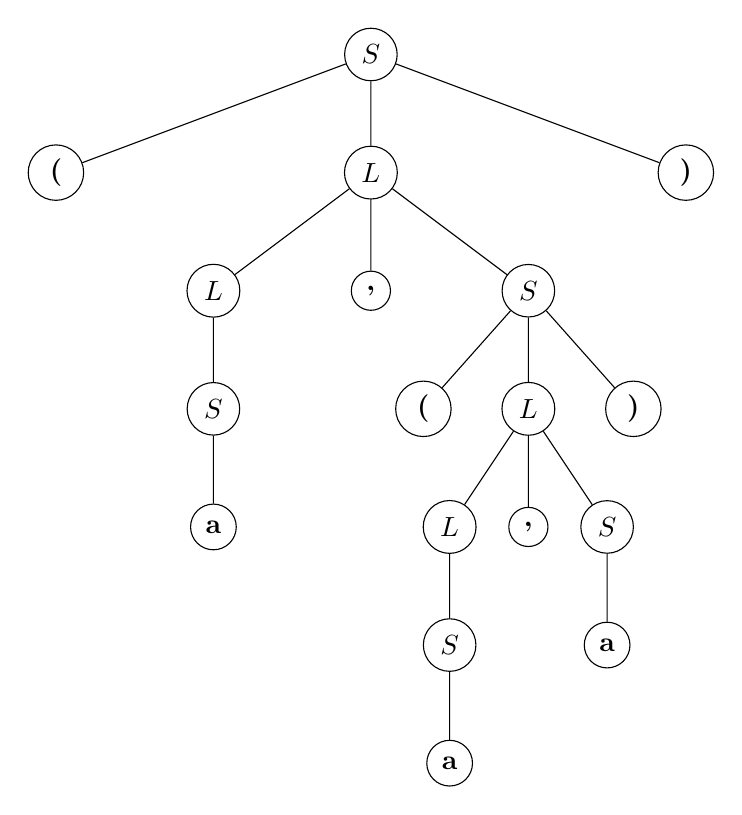
\begin{tikzpicture}[level/.style={sibling distance=40mm/#1}]
\node [circle,draw] 
 (root){$S$}
 	child {node [circle,draw] (root_1) {\textbf{(}}}
	child {node [circle,draw] (root_2) {$L$}
		child {node [circle,draw] (root_21) {$L$}
			child {node [circle,draw] (root_211) {$S$}
				child {node [circle,draw] (root_2111) {\textbf{a}}}
			}
		}
		child {node [circle,draw] (root_22) {\textbf{,}}}
		child {node [circle,draw] (root_23) {$S$}
			%hijo identico al inciso anterior
			child {node [circle,draw] (root_231) {\textbf{(}}}
			child {node [circle,draw] (root_232) {\textbf{$L$}}				
				child {node [circle,draw] (root_2321) {$L$}
					child {node [circle,draw] (root_23211) {$S$}
						child {node [circle,draw] (root_232111) {\textbf{a}}}
					}
				}
				child {node [circle,draw] (root_2322) {\textbf{,}}}
				child {node [circle,draw] (root_2323) {$S$}
					child {node [circle,draw] (root_23231) {\textbf{a}}}
				}
			}
			child {node [circle,draw] (root_233) {\textbf{)}}}
		}
	}
	child {node [circle,draw] (root_3) {\textbf{)}}};
\end{tikzpicture}
\end{center}

\end{itemize}
\end{homeworkProblem}

%%% Problema 2
\begin{homeworkProblem}[Problema 2]
\subsection{Construya un DFA que acepte los siguientes lenguajes sobre el alfabeto $\{0,1\}$}
\begin{itemize}

%item 1
\item Conjunto de cadenas que terminen en 00 \\

\begin{center}
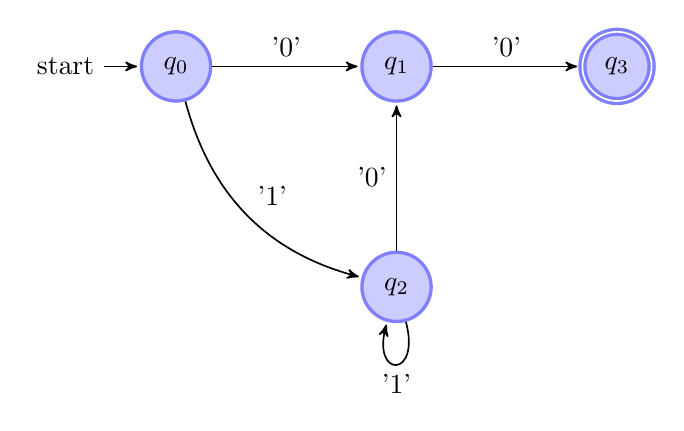
\begin{tikzpicture}[->,>=stealth',shorten >=1pt,auto,node distance=2.8cm,semithick]
  \tikzstyle{every state}=[draw=blue!50,very thick,fill=blue!20]

  \node[initial,state] 	(A)                    {$q_0$};
  \node[state]          	(B) 	[right of=A] {$q_1$};
  \node[state]         	(C) 	[below of=B] {$q_2$};
  \node[state,accepting]         	(D) 	[right of=B] {$q_3$};

  \path 	(A) 	edge  		node {'0'} (B)
  		(A)	edge	 [bend right]	node {'1'} (C)
		(C)	edge [loop below]	node {'1'}(C)
		(C)	edge	 			node {'0'} (B)
		(B)	edge	 		node {'0'} (D);
\end{tikzpicture}
\end{center}

%item 2
\item Conjunto de cadenas con tres 0 consecutivos (no necesariamente al final) \\

\begin{center}
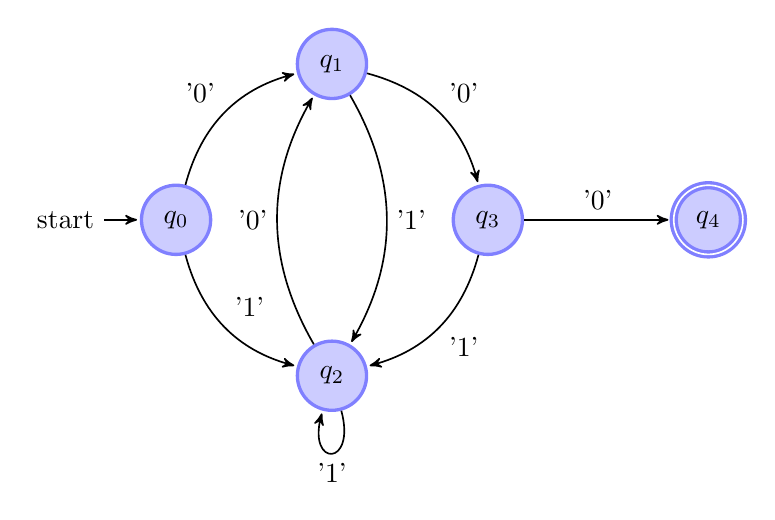
\begin{tikzpicture}[->,>=stealth',shorten >=1pt,auto,node distance=2.8cm,semithick]
  \tikzstyle{every state}=[draw=blue!50,very thick,fill=blue!20]

  \node[initial,state] 	(A)                   			 {$q_0$};
  \node[state]		(B)	[above right of =A]	 {$q_1$};
  \node[state]		(C)	[below right of =A]	{$q_2$};
  \node[state]		(D)	[below right of =B]	{$q_3$};
  \node[state,accepting] (E)[right of =D]		{$q_4$};
				
  \path 			(A)	edge		[bend left]		node {'0'}	(B)
  				(A)	edge		[bend right]	node {'1'} 	(C)
				(C)	edge		[loop below]	node {'1'}	(C)
				(C)	edge		[bend left]		node {'0'}	(B)
				(B)	edge		[bend left]	node {'1'} 	(C)
				(B)	edge		[bend left]		node {'0'} 	(D)
				(D)	edge		[bend left]	node {'1'}	(C)
				(D)	edge					node {'0'}	(E);
\end{tikzpicture}
\end{center}

%item 3
\item Conjunto de cadenas que empiecen con 01\\

\begin{center}
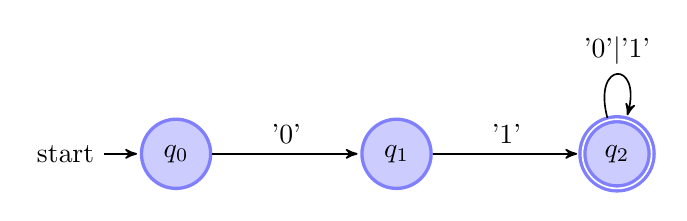
\begin{tikzpicture}[->,>=stealth',shorten >=1pt,auto,node distance=2.8cm,semithick]
  \tikzstyle{every state}=[draw=blue!50,very thick,fill=blue!20]

  \node[initial,state] 	(A)                   			 {$q_0$};
  \node[state]		(B)	[right of =A]		{$q_1$};
 \node[state,accepting]		(C)	[right of =B]		{$q_2$};
 
 \path			(A)	edge		node{'0'}	(B)	
 				(B)	edge		node{'1'}	(C)
				(C)	edge [loop above] node{'0'$|$'1'} (C);
 
\end{tikzpicture}
\end{center}

%item 4
\item Conjunto de cadenas que contengan a 001 como sub-cadena\\

\begin{center}
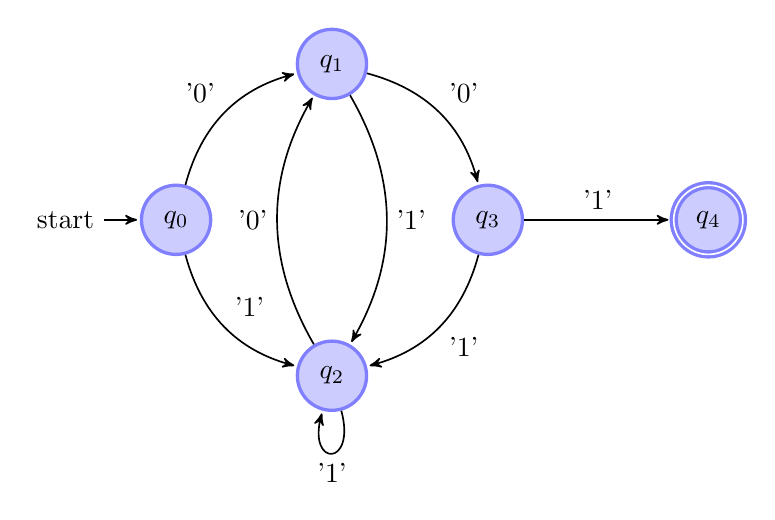
\begin{tikzpicture}[->,>=stealth',shorten >=1pt,auto,node distance=2.8cm,semithick]
  \tikzstyle{every state}=[draw=blue!50,very thick,fill=blue!20]

  \node[initial,state] 	(A)                   			 {$q_0$};
  \node[state]		(B)	[above right of =A]	 {$q_1$};
  \node[state]		(C)	[below right of =A]	{$q_2$};
  \node[state]		(D)	[below right of =B]	{$q_3$};
  \node[state,accepting] (E)[right of =D]		{$q_4$};
				
  \path 			(A)	edge		[bend left]		node {'0'}	(B)
  				(A)	edge		[bend right]	node {'1'} 	(C)
				(C)	edge		[loop below]	node {'1'}	(C)
				(C)	edge		[bend left]		node {'0'}	(B)
				(B)	edge		[bend left]	node {'1'} 	(C)
				(B)	edge		[bend left]		node {'0'} 	(D)
				(D)	edge		[bend left]	node {'1'}	(C)
				(D)	edge					node {'1'}	(E);
\end{tikzpicture}
\end{center}	
\end{itemize}
\end{homeworkProblem}

\begin{homeworkProblem}[Problema 3]
\subsection{Escriba expresiones regulares para los lenguajes del ejercicio anterior}

\begin{itemize}
\item Conjunto de cadenas que terminen en 00 \\
\textbf{Respuesta:} \[  (0|1)^*00\]
\item Conjunto de cadenas con tres 0 consecutivos (no necesariamente al final) \\
\textbf{Respuesta:} \[  (0|1)^*000(0|1)^*\]
\item Conjunto de cadenas que empiecen con 01\\
\textbf{Respuesta:} \[  01(0|1)^*\]
\item Conjunto de cadenas que contengan a 001 como sub-cadena\\
\textbf{Respuesta:} \[  (0|1)^*001(0|1)^*\]

\end{itemize}

\end{homeworkProblem}

\begin{homeworkProblem}[Problema 4]
\subsection{De una descripci\'{o}n del lenguaje que generan las siguientes expresiones regulares}

\begin{itemize}
\item $L = (0^*1^*)^*000(0|1)^*$\\

Digamos que $L$ est\'{a} conformado por tres partes de manera que $L = L_1L_2L_3$ i.e. $L_1,L_2$ y $L_3$ son sub-cadenas de $L$ las cuales se concatenan entre s\'{i} obligatoriamente en el orden establecido.

Observemos que $L_2$ es en s\'{i} es, tres ceros 'obligatorios', es decir, que todas las cadenas $w \in L$ tendr\'{a}n a tres ceros $(L_2)$ como sub-cadena, en alguna parte entre el inicio y el final.

Para definir la sub-cadena que representa $L_1$ al principio de cada cadena en $L$, observemos que la expresi\'{o}n $0^*$ genera a $\epsilon | 0 | 00 | 000 \dots$ y $1^*$ denota al lenguaje cuyas cadenas son $\epsilon | 1 | 11 | 111 \dots$. Notemos entonces que $L_1 = (0^*1^*)^*$ denota al lenguaje con las cadenas resultantes de concatenar alguna cadena generada por $0^*$ seguida por una generada por $1^*$ cero o m\'{a}s veces.

Las sub-cadenas que representa $L_3$ al final de $L$ son el conjunto de concatenar ninguna o m\'{a}s veces un 0 o un 1, e.g. $\epsilon | 0 | 1 | 00 | 01 | 10 | 11 | \dots $, es decir, todos los n\'{u}meros binarios posibles y $\epsilon$.

\textbf{Ejemplos de cadenas $\in L$}
\begin{itemize}
\item $00110011 000 00110101$ en donde $L_1 = 00110011$, $L_2 = 000$ como siempre y $L_3 = 00110101$
\item $000 0101010111$ en donde $L_1 = \epsilon$, $L_2 = 000$ como siempre y $L_3 = 0101010111 $
\end{itemize}

\item $(0|10)^*1^*$\\

An\'{a}logamente, pensando en $L$ como una concatenaci\'{o}n de dos lenguajes $L_1$ y $L_2$, tenemos $L=L_1L_2$ en ese orden espec\'{i}fico. 

$L_1$ contiene las sub-cadenas de $L$ al principio que resultan de concatenar cero o m\'{a}s veces un 0 con un 10 o viceversa, es decir, un 10 con un 0. Por ejemplo: 010 \'{o} 100. Esta generaci\'{o}n de cadenas ser\'{i}a $\epsilon | 0 | 10 | 010 | 100 \dots$.

$L_2$ contiene las subcadenas de $L$ al final, que es el resultado de concatenar 1 cero o m\'{a}s veces i.e. $\epsilon | 1 | 11 | 111 | 1111$.

\textbf{Ejemplos de cadenas $\in L$}
\begin{itemize}
\item $10101010 1111$ en donde $L_1 = 10101010 $ y $L_2 = 1111$
\item $000010$ en donde $L_1 = 000010 $ y $L_2 = \epsilon$ 
\end{itemize}
\end{itemize}
\end{homeworkProblem}


\begin{homeworkProblem}[Problema 5]
\subsection{Dadas dos expresiones regulares $r_1$ y $r_2$. C\'{o}mo demostrar\'{i}a (o refutar\'{i}a) que $L(r_1) = L(r_2)$}

Dado que las expresiones regulares se definen recursivamente, sabiendo que $r_1$ y $r_2$ son expresiones regulares entonces tenemos:

\begin{itemize}
\item $L(r_1|r_2) = L(r_1) \cup L(r_2)$
\item $L(r_1r_2) = L(r_1) L(r_2)$
\item $L(r_1^*) = (L(r_1))^*$
\item $L((r_1)) = L(r_1)$
\end{itemize}

La respuesta ser\'{i}a hacer la serie de pasos recursivos hasta que lleven al lenguaje en una expresi\'{o}n denotada con las expresiones regulares anteriormente mencionadas.

Tomemos como ejemplo la siguiente demostraci\'{o}n dadas dos expresiones regulares.

Dados $L = \{$ todas las cadenas sin dos 0 consecutivos$\}$, $r_1 = (1|01)^*(0|\epsilon)$ y $r_2 = (1^*011^*)(0|\epsilon) | 1^*(0|\epsilon)$. Demostremos que $L(r_1) = L(r_2) = L$ \\

Veamos que

\[  L(r_1) = L( (1|01)^*(0 |\epsilon) )\]

\[ L(  (1|01)^* )   L( 0|\epsilon )\]

\[ L(  (1|01) )^*   L( 0 ) \cup L(\epsilon)\]

\[ L(  L(1) \cup L(01)     )^*   (\{ 0\} \cup \{ \epsilon \} )\]

\[ (\{1\} \cup \{01\})^*   (\{ 0,\epsilon \} )\]

\[ \{1,01,11,011, 101, 0101 \dots \}   (\{ 0,\epsilon \} )\]

\[ \{ \epsilon,0,10,010,110,0110, 1010, 01010, \dots, 1,01,11,011, 101, 0101  \}  \]

efectivamente vemos que $L(r_1) = L$

Ahora, 

\[ L(r_2) =   L(  (1^*011^*)   (\epsilon|0)     )  |  1^*(\epsilon|0) )   \]

\[  L(   L((1^*011^*))   L(\epsilon|0)    )  \cup  L(1^*(\epsilon|0))  \]

\[  L(   L(1^*) L(011^*)       (L(0) \cup L(\epsilon))   \cup  L(   L(1^*)    (  L(\epsilon ) \cup L(0))    )        )   \]

\[  \set{1}^* (\set{011}^*)  (\set{\epsilon,0})    \cup   \set{1}^* (\set{\epsilon,0}) \]

Para mayor legibilidad del lector, notemos que ${1}^*$ act\'{u}a como lenguaje operando al principio en los dos conjuntos que ser\'{a}n unidos, entonces escribimos

\[  \set{1}^*  [   (\set{011}^*) (\set{\epsilon,0}) \cup) \cup \set{\epsilon,0} ]\]

Observemos ahora que el segundo conjunto a ser unido, $ \set{\epsilon,0}  $, ya est\'{a} contenido en el primero. Entonces,

\[ \set{1}^*    (  \set{ 011}^* \set{\epsilon,0} )      \]

\[ \set{\epsilon,1,11,111,111\dots}^*   (\set{\epsilon,0,011,0110,011011,0110110\dots  })  \]

\[ \set{\epsilon, 0, 011,0110,011011,0110110,\dots, 10, 1011,10110,1011011,10110110\dots}\]

el cual tambi\'{en} es el mismo conjunto que $L$ y $L(r_1)$, implicando que $L(r_1)=L(r_2)=L$
\end{homeworkProblem}

\begin{homeworkProblem}[Problema 6]
\subsection{Sea $w = xy$ donde $x$ y $y$ son cadenas sobre un conjunto de s\'{i}mbolos dados. Demuestre que $\hat{\delta}(q,xy) = \hat{\delta}(\hat{\delta}(q,a),y)$, donde $\hat{\delta}$ es la funci\'{o}n de transici\'{o}n extendida definida para un AFD. }

Por inducci\'{o}n tenemos como caso base:
Si $y = \epsilon$, entonces 
\[ \hat{\delta}(q,x) = \hat{\delta}(\hat{\delta}(q,x),\epsilon) \]

Que cumple para la definici\'{o}n de $\hat \delta$

\textbf{Paso inductivo:} Asumimos que la proposici\'{o}n se cumple para cadenas m\'{a}s peque\~{n}as  y partimos $y = wa$, en donde $a$ es el \'{u}ltimo s\'{i}mbolo de $y$.

Partamos entonces de $\hat \delta ( \hat \delta(q,x) ,y   )$, que por la separaci\'{o}n de $y$ se convierte en

\[ \hat \delta ( \hat \delta(q,x) ,wa )\]

Por la definici\'{o}n de $\hat \delta$, sabemos que eso es lo mismo que

\[ \delta (  \hat \delta ( \hat \delta(q,x) ,w )       ,a ) \]

Y por nuestra hip\'{o}tesis inductiva,

\[ \delta (  \hat \delta(q,xw)   ,a)\]

De nuevo, por la definici\'{o}n de $\hat \delta$ tenemos

\[ \hat \delta (q,xwa)\]

Y por la separaci\'{o}n que hicimos de $y$ en $wa$, tenemos

\[ \hat \delta ( q,xy)\]

\qed 
\end{homeworkProblem}

\begin{homeworkProblem}[Problema 7]
\subsection{Demuestre que para cualquier estado $q$, cadena $x$ y s\'{i}mbolo de entrada $a$ tenemos que $\hat{\delta}(q,ax) = \hat{\delta}(\delta(q,a),x)$, donde $\delta$ es la funci\'{o}n de transici\'{o}n y $\hat{\delta}$ es la funci\'{o}n de transici\'{o}n extendida para un AFD.}


\end{homeworkProblem}

\begin{homeworkProblem}[Problema 8]
\subsection{Dada una especificaci\'{o}n de componentes l\'{e}xicos, explique: C\'{o}mo a partir de dicha especificaci\'{o}n se puede generar un analizador l\'{e}xico que reconozca dicha especificaci\'{o}n i.e. que reconozca cada uno de los componentes l\'{e}xicos?}

Tenemos una especififaci\'{o}n de componentes l\'{e}xicos en forma de expresiones regulares $r_1,r_2\dots r_n$. Usando el algoritmo de Thompson generar\'{i}a un Automata No-Determinista $\epsilon-AFN_1,\epsilon-AFN_2\dots\epsilon-AFN_3$con transiciones $\epsilon$ para cada expresi\'{o}n regular.

Luego usando el algoritmo de cerradura-$\epsilon$ convertir\'{i}a cada $\epsilon-AFN_i$ en una serie de Automatas No-Deterministas $AFN_1,AFN_2\dots AFN_n$. Luego con el algoritmo de construcci\'{p}n de subconjuntos convertir\'{i}a cada $AFN_i$ en un Automata Finito Determinista.

En este punto, tenemos $n$ Automatas Finitos Deterministas, uno para cada expresion regular. Por \'{u}ltimo, compondr\'{i}a UN SOLO Automata No-Determinista con transiciones $\epsilon$, eso es:

\begin{center}
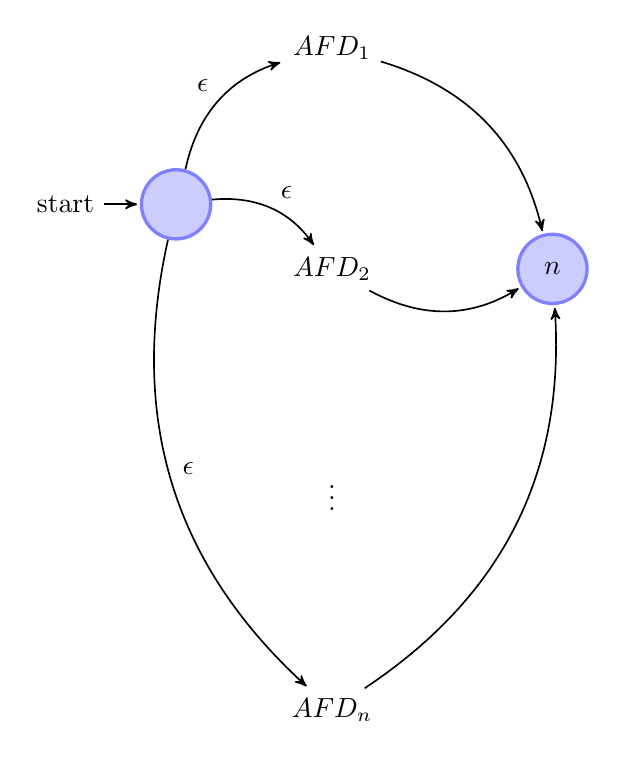
\begin{tikzpicture}[->,>=stealth',shorten >=1pt,auto,node distance=2.8cm,semithick]
  \tikzstyle{every state}=[draw=blue!50,very thick,fill=blue!20]

  \node[initial,state] 	(A)                   			 {};
  \node			(B)	[above right of =A]	 {$AFD_1$};
  \node			(C)	[below of =B]	{$AFD_2 $};
  \node			(D)	[below of =C]	{$\vdots$};
  \node			(E) 	[below of =D]	{$AFD_n$};
  \node[state]		(F)	[right of =C]	{$n$};		
				
  \path			(A)	[bend left] 	 edge node{$\epsilon$} 	(B)		
  				(A)			 edge node{$\epsilon$} 	(C)
				(A)	[bend right] 	 edge node{$\epsilon$} 	(E)
				(B)	edge [bend left] 		(F)
				(C)	edge 	 		(F)
				(E)	edge [bend right] 		(F);
\end{tikzpicture}
\end{center}	

Teniendo este Automata grande, aplicar\'{i}a de nuevo cerradura-$\epsilon$ y construcci\'{o}n de subconjuntos para llegar a un solo Automata Finito Determinista $A$.

Con $A$ podemos rechazar o aceptar a cualquier cadena en la especificacion de componentes l\'{e}xicos.


\end{homeworkProblem}

\begin{homeworkProblem}[Investigue: Complejidad Computacional y An\'{a}lisis de Algoritmos]

\subsection{Qu\'{e} es complejidad computacional?}
Complejidad computacional es una rama de la teor\'{i}a de la computaci\'{o}n que se enfoca en clasificar problemas computacionales acorde a su dificultad. En este contexto, se entiende que un problema est\'{a} sujeto a ser resuelto por una computadora.

\subsection{Automata Finito}
Un automata finito toma una cadena de entrada y devuelve una respuesta de la forma "aceptado" o "rechazado", eso es:

\tikzstyle{int}=[draw, fill=blue!15, minimum size=2em]
\tikzstyle{init} = [pin edge={to-,thin,black}]

\begin{center}
\begin{tikzpicture}[node distance=4.5cm,auto,>=latex']
    \node [int, pin={[init]above:Cadena:$String$}] (a) {Automata Finito};
    \node (b) [left of=a,node distance=4.5cm, coordinate] {a};
    \node [init] (c) [right of=a] {"Aceptado" o "Rechazado"};
    \node [coordinate] (end) [right of=c, node distance=2cm]{};
    \path[->] (a) edge node {} (c) ;
\end{tikzpicture}
\end{center}

La definici\'{o}n formal de un Automa Finito $M$ es $M = (Q,\sum{},\delta,q_0F)$ en donde:
\begin{itemize}
\item $Q$: conjunto de estados
\item $\sum{}$ : alfabeto de entrada
\item $\delta$: funci\'{o}n de transici\'{o}n
\item $q_0$: estado de transici\'{o}n
\item $F$: conjunto de estados de aceptaci\'{o}n
\end{itemize}

\subsection{Lenguaje aceptados por Automatas Finitos}
Definimos a $L(M)$ como el lenguaje que contiene todas las cadenas aceptadas por un automata finito $M$

Ejemplo:
$L(M) = \set{abba}$
\vspace{-1cm}
\begin{center}
\[ M \]
\ovalbox{
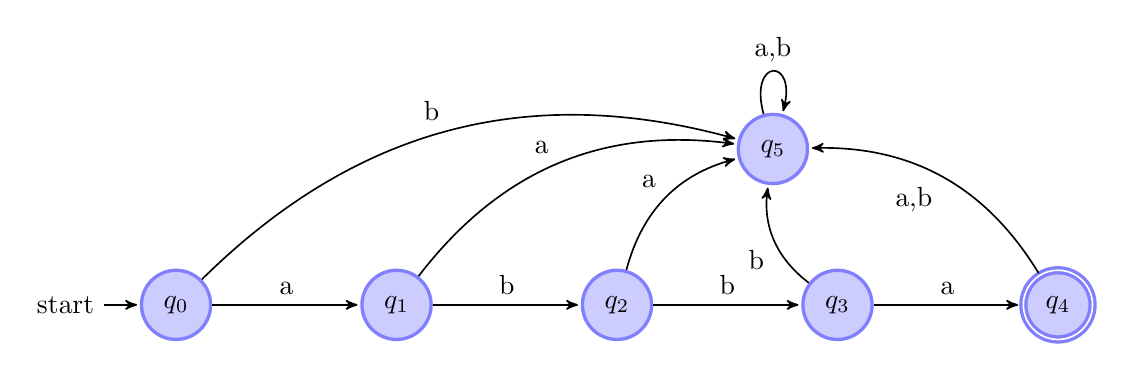
\begin{tikzpicture}[->,>=stealth',shorten >=1pt,auto,node distance=2.8cm,semithick]
  \tikzstyle{every state}=[draw=blue!50,very thick,fill=blue!20]

  \node[initial,state] 	(A)                    {$q_0$};
  \node[state]          	(B) 	[right of=A] {$q_1$};
  \node[state]         	(C) 	[right of=B] {$q_2$};
  \node[state]         	(D) 	[right of=C] {$q_3$};
  \node[state,accepting]         	(E) 	[right of=D] {$q_4$};
  \node[state]         	(F) 	[above right of=C] {$q_5$};
  

  \path 	(A) 	edge  		node {a} (B)
  		(B)	edge	 		node {b} (C)
		(C)	edge 		node {b}(D)
		(D)	edge	 		node {a} (E)
		(A)	edge	 [bend left] node{b} (F)
		(B)	edge	 [bend left] node{a} (F)
		(C)	edge	 [bend left] node{a} (F)
		(D)	edge	 [bend left] node{b} (F)
		(E)	edge	 [bend right]node{a,b} (F)
		(F) 	edge [loop above] node{a,b} (F)
		;
\end{tikzpicture}}
\end{center}

En donde
\begin{itemize}
\item $Q = \set{q_0,q_1,q_2,q_3,q_4,q_5}$
\item $\sum{} = \set{a,b}$
\item $\delta$: funci\'{o}n de transici\'{o}n, en donde aparecen $\delta(q_0,a) = q_1, \delta(q_0,b) = q_5 \dots$
\item $q_0$ es el estado inicial
\item $F = \set{q_4}$
\end{itemize}


\subsection{Lenguajes Regulares}
Decimos que un lenguaje $L$ es regular si existe un automata finito $M$ tal que $L = L(M)$, eso es, que el automata finito pueda generar a $L$.

Observaci\'{o}n: Todos los lenguajes aceptados por Automatas Finitos, forman la familia de los Lenguajes Regulares.


Ejemplos de lenguajes regulares:
\begin{itemize}
\item \set{abba} 
\item \set{$\epsilon$,ab,abba}
\item \set{\text{todas las cadenas que empiezan con $ab$}}
\end{itemize}


\subsection{Gram\'{a}tica independiente del contexto}
Decimos que $G$ es una gram\'{a}tica independiente si es de la forma $G = (V,T,S,P)$ en donde:

\begin{enumerate}
\item $T$ es un conjunto de \textbf {terminales}
\item $V$ es un conjunto de \textbf{no terminales } (variables sin\'{a}cticas)
\item $P$ es el conjunto de producciones de la forma $A -> x$
\item $S$ es una definici\'{o}n de un \textbf{no terminal} como s\'{i}mbolo inicial de $G$.
\end{enumerate}

\textbf{Ejemplo, $G$:} \\
\indent \indent $L -> L $ '+' $d$\\
\indent \indent $L -> L $ '-' $d$\\
\indent \indent $L -> d$\\
\indent \indent $L -> '0' || '1' || '2' ... '9' $\\

En donde el s\'{i}mbolo inicial es el \textbf{no terminal} $L$.\\ 

\indent \indent $L -> L $ '+' $d$ (Regla 1) \\
\indent \indent $L -> d $ '+' $d$ (Regla 3)\\
\indent \indent $L -> 5 $ '+' $d$ (Regla 4) \\
\indent \indent $L -> 5 $ '+' $1$ (Regla 4) \\

Y decimos que $w \in L(G)$

\subsection{Lenguajes libres de contexto}
Decimos que un lenguaje $L$ es libre de contexto s\'{i} y solo si existe una gram\'{a}tica $G$ con $L=L(G)$, eso es $L(G) = \{ w | w \text{ es derivada a partir de $G$}\}$, que es el conjunto de todas las producciones posibles a partir de $G$ \\

\subsection{M\'{a}quina de Turing}
Una m\'{a}quina de Turing es un modelo matem\'{a}tico de una m\'{a}quina computacional. Es un dispositivo que manipula s\'{i}mbolos contenidos en una cinta y se cree que si un problema puede ser resuelto por un algoritmo, entonces existe una m\'{a}quina de Turing que puede resolver el problema. En la teor\'{i}a computacional es el modelo de computadora m\'{a}s utilizado. Nos enfocaremos en este.

Conceptualmente, una m\'{a}quina de Turing, como un Automata Finito, consiste de un control finito y una cinta. A cualquier hora est\'{a} en uno de los estados finitos. La cinta se extiende infinitamente hacia la derecha y tambi\'{e}n est\'{a} dividido en cuadrados en los cuales puede ser escrito un s\'{i}mbolo. Aunque, a diferencia de los automatas finitos, su cabeza puede leer y escribir y se puede mover hacia la izquierda, derecha o quedarse en el mismo cuadrado despu\'{e}s de haber le\'{i}do o escrito.

\begin{center}
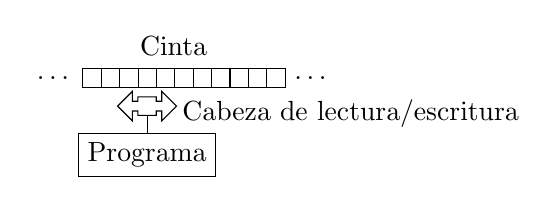
\begin{tikzpicture}[
      start chain=1 going right,start chain=2 going below,node distance=-0.15mm
    ]
    \node [on chain=2] {Cinta};
    \node [on chain=1] at (-1.5,-.4) {\ldots};  
    \foreach \x in {1,2,...,11} {
        \x, \node [draw,on chain=1] {};
    } 
    \node [name=r,on chain=1] {\ldots}; 
    \node [name=k, arrow box, draw,on chain=2,
        arrow box arrows={east:.25cm, west:0.25cm}] at (-0.335,-.65) {};    
    \node at (2.25,-.85) {Cabeza de lectura/escritura};
    \node [on chain=2] {};
    \node [draw,on chain=2] {Programa};
    \chainin (k) [join]; % Verbindung vom Programm zum Leseschreibkopf
\end{tikzpicture}
\end{center}

Dada una cadenea de s\'{i}mbolos en una cinta, una m\'{a}quina de Turing empieza en el estado inicial. En cualquier estado, la cabeza lee el s\'{i}mbolo bajo ella y puede ya sea borrarlo o remplazarlo con otro s\'{i}mbolo (posiblemente el mismo). Despu\'{e}s mueve la cabeza hacia la izquierda o derecha o no se mueve y procede al siguiente estado, que puede ser el mismo que el actual. Uno de sus estados es el estado en donde la computaci\'{o}n para y cuando la m\'{a}quina de Turing para.

Formalmente, una m\'{a}quina de Turing es una 5-tupla $M = (Q,\sum,\Gamma,q_0,\delta)$ en donde:
\begin{itemize}
\item $Q$ es un conjunto finito de estados, en donde se asume que ninguno contiene al s\'{i}mbolo $h$. El s\'{i}mbolo $h$ se usa para denotar al estado de interrupci\'{o}n.
\item $\sum$ es un conjunto finito de s\'{i}mbolos y el alfabeto de entrada.
\item $\Gamma$ es un conjunto finito de s\'{i}mbolos conteniendo $\sum$ como subconjunto y es el conjunto de s\'{i}mbolos en la cinta.
\item $q_0$ es el estado inicial
\item $\delta$ es la funci\'{o}n de transici\'{o}n pero su valor puede no estar definido para ciertos puntos, es un mapeo desde $Q \times (\Gamma \cup \set{V})$ a $(Q \cup \set{h}) \times (\Gamma \cup \set{\Delta}) \times \set{R,L,S}$.

Aqu\'{i} $\Delta$ denota el vac\'{i}o y $R,L$ y $S$ denotan una movida de la cabeza hacia la derecha, izquierda o la misma (sin moverla) respectivamente.  
\end{itemize}

\subsection{Aceptancia en una m\'{a}quina de Turing}
Una m\'{a}quina de Turing $M$ acepta a la entrada si la m\'{a}quina se para o se interrumpe en un estado final.

La misma m\'{a}quina de Turing rechaza la entrada si la m\'{a}quina para o se interrumpe en un estado no-final, o si la m\'{a}quina entra en un ciclo infinito.

\subsection{Definici\'{o}n de un algoritmo}
Un algoritmo para la funci\'{o}n $f(w)$ es una m\'{a}quina de Turing que computa $f(w)$. Esto es en efecto, la t\'{e}sis de Alan Turing, los algoritmos son m\'{a}quinas de Turing. Cuando existe 'existe un algoritmo' nos referimos a 'existe una m\'{a}quina de Turing que ejecuta el algoritmo'.

\subsection{M\'{a}quina de Turing determinista}
En una m\'{a}quina de Turing determinista, que es uno de los modelos m\'{a}s usados para definir clases de complejidad, no est\'{a} permitido tener una funci\'{o}n de transici\'{o}n que para un mismo estado dado y un s\'{i}mbolo, solo tiene un movimiento de respuesta i.e. derecha, izquierda o quedarse en el mismo cuadro.

Existen otros modelos de m\'{a}quina de Turing, como la m\'{a}quina de turing no-determinista, la m\'{a}quina de Turing cu\'{a}ntica, la m\'{a}quina de Turing sim\'{e}trica, m\'{a}quina de Turing probabilistica o una m\'{a}quina de Turing alternante. Todas ellas son igualmente capaces en principio de computar un algoritmo pero cuando los recursos (como el tiempo o el espacio) est\'{a}n limitados, algunas de estas pueden ser m\'{a}s poderosas que otras.

\subsection{Lenguajes aceptados por m\'{a}quinas de Turing}
Una m\'{a}quina de Turing acepta a los lenguajes independientes del contexto y a los lenguajes regulares, que est\'{a}n contenidos en los lenguajes independientes del contexto. Tambi\'{e}n aceptan unos lenguajes que no definimos aqu\'{i} que son de la forma $a^nb^nc^n$ y $ww$.

\subsection{Medidas de complejidad}
Para una definici\'{o}n m\'{a}s precisa de que significa resolver un problema dado una cantidad de recursos (tiempo o espacio), un modelo computacional como una m\'{a}quina de Turing puede ser usada. El $tiempo$ requerido por una m\'{a}quina de Turing determinista $M$ para una entrada $x$ es el n\'{u}mero total de transiciones de estado, o el n\'{u}mero de pasos que esta hace antes de interrumpirse y dar salida a la respuesta ("si" o "no").

Se dice que una m\'{a}quina de Turing $M$ opera en un tiempo de $f(n)$ si el tiempo requerido por $M$ para cada entrada de longitud $n$ es a lo sumo $f(n)$. Un problema de decisi\'{o}n $A$ puede ser resuelto en tiempo $f(n)$ si existe una m\'{a}quina de Turing que opera en tiempo $f(n)$ que resuelve el problema.

La teor\'{i}a  de complejidad computacional se enfoca en separar y clasificar problemas basados en su dificultad, se definen conjuntos de problemas basados en cierto criterio. Por ejemplo, el conjunto de los problemas resolvibles en un tiempo $f(n)$  en una m\'{a}quina de Turing determinista  es denotado DTIME$(f(n))$ y es una clase de complejidad.

\subsection{El recurso DTIME$(n)$}
Usando la notaci\'{o}n $O(k)$, usaremos una m\'{a}quina de Turing con multicintas y contaremos el n\'{u}mero de pasos hasta que una cadena sea aceptada. 

Ejemplo: $L = \set{a^nb^n:n \geq 0 }$
Algoritmo que acepta una cadena $w$:
\begin{itemize}
\item Usamos una m\'{a}quina de Turing de dos cintas
\item Copiamos $a$ en la segunda cinta
\item Comparamos $a$ y $b$
\end{itemize}

El tiempo necesitado para computar la salida de $w$ es:
\begin{itemize}
\item Copiamos $a$ en la segunda cinta $\implies$ \indent \indent $O(|w|)$
\item Comparamos $a$ y $b$ $\implies$ \indent \indent $O(|w|)$
\end{itemize}

Tiempo total necesitado: $O(|w|)$\\

Eso es, para una cadena de longitud $n$, el tiempo necesitado para ser aceptado es de $O(n)$

Decimos entonces que la clase de complejidad del lenguaje es DTIME$(n)$ dado que una m\'{a}quina de Turing determinista acepta cada cadena de longitud $n$ en tiempo $O(n)$

De una manera similar, definimos la clase DTIME$(T(n))$ para cualquier funci\'{o}n de tiempo $T(n)$, por ejemplo: DTIME$(n^2)$, DTIME$(n^3),\dots$\\

\textbf{Teorema:}
DTIME$(n^{k+1}) \text{contiene a DTIME}(n^k)$

Decimos que los algoritmos con tiempo polinomial son DTIME$(n^k)$ y para un $k$ pequeno podemos computar el resultado r\'{a}pido

\subsection{La clase $P$}
La clase $P$ est\'{a} definida como 

\[ P = \cup \text{DTIME}(n^k) \text{ para todo $k$}\] 
\begin{itemize}

\subsection{}
\item Tiene tiempo polinomial
\item Contiene todos los problemas con tiempo polinomial.
\end{itemize}

\subsection{Otras clases}
Existen otras clases de complejidad, pero las m\'{a}s importantes son generalmente definidas por limitar el tiempo o el espacio usado por el algoritmo. 



\subsection{An\'{a}lisis de algoritmos}
El analizar un algoritmo significa determinar la cantidad de recursos (como tiempo y espacio) necesarios para ejecutarlo.  Es una parte de la amplia teor\'{i}a de la complejidad computacional, explicada anteriormente.

En el an\'{a}lisis de algoritmos, es com\'{u}n estimar su complejidad en un \textbf{sentido asint\'{o}tico} i.e. estimar la funci\'{o}n de complejidad para una entrada grande. Aqu\'{i} notaciones como la Big $O$ (usada para definir $P$ en el inciso anterior), $\Omega$ y $\Theta$ son usadas para este fin.

Por ejemplo, un algoritmo de b\'{u}squeda binaria corre en un n\'{u}mero de pasos proporcionales al logaritmo de el tamano de la lista en donde se est\'{a} buscando i.e. $O(\log(n))$, dicho comunmente "en tiempo logaritmico"

\end{homeworkProblem}

\subsection{Notaci\'{o}n Big-$O$}
Algunas veces en an\'{a}lisis de el tiempo de corrida de los algoritmos, se puede ser muy dejado   y esto podr\'{i}a llevar a un nivel de inexactitud en el resultado. Pero tambi\'{e}n el riesgo opuesto est\'{a} presente: es posible ser $demasiado$ preciso. Un an\'{a}lisis profundo se basa en las simplificaciones correctas.

El expresar el tiempo en t\'{e}rminos de \textit{pasos b\'{a}sicos de computadora} es ya una simplificaci\'{o}n. Despu\'{e}s de todo, el tiempo tomado para cada una de esos pasos depende en el procesador y hasta en los detalles de como hacer $cache$ y como resultado, el tiempo de corrida podr\'{i}a diferir entre una ejecuci\'{o}n de un algoritmo con otra.

Es necesario entonces, expresar la eficiencia de un algoritmo en t\'{e}rminos que sean independientes de la m\'{a}quina en donde est\'{a} corriendo. Y esto lleva a otra simplificaci\'{o}n, en vez de decir que un algoritmo toma $8n^3 + 2n + 10$ pasos para una entrada de tamano $n$, es mucho m\'{a}s simple creer que los t\'{e}rminos m\'{a}s bajos como $2n$ y $10$ (que ser\'{a}n insignificantes mientras $n$ crezca), y hasta el detalle del coeficiente 8 en el primer t\'{e}rmino, decimos que el algoritmo corre en tiempo $O(n^3)$.

Es en efecto el tiempo que define esta notaci\'{o}n precisamente. Pensemos en $f(n)$ y $g(n)$ como tiempos de corrida de dos algoritmos con la misma entrada de tamano $n$.

Sean $f(n)$ y $g(n)$ funciones que van de los enteros positivos hacia los reales positivos. Decimos que $f = O(g)$, que significa que $f$ no crece m\'{a}s r\'{a}pido que $g$, si hay una constante $ c > 0$ que cumpla con $f(n) \leq c\cdot g(n)$

Entonces, tenemos una herramienta para elegir digamos entre dos algoritmos que corren uno en $f_1(n) = n^2$ pasos y el otro $f_2(n) = 2n+20)$. Si graficamos las dos notemos que

\begin{center}
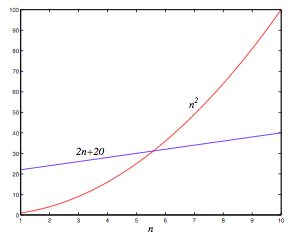
\includegraphics[width=7cm]{bigo.png}
 \end{center}

para $n \leq 5$, $f_1$ es mas pequeno. En este caso, $f_2$ se escala mucho mejor mientras $n$ crece y por eso es superior. Esto es capturado por la notaci\'{o}n big-$O$: $f_2 = O(f_1)$, ya que:

\[ \frac{f_2(n)}{f_1(n)} = \frac{2n+20}{n^2} \leq 22\] 

para todo $n$; de otro modo, vemos que $f_1 \neq O(f_2)$, ya que $f_1(n) / f_2(n) = n^2 / (2n+20)$ puede ser arbitrariamente largo y por lo tanto no hay ninguna constante $c$ tal que cumpla la definici\'{o}n.

\begin{homeworkProblem}[Investigue: Generadores de Analizadores L\'{e}xicos]
Un generador de analizadores l\'{e}xico, hace lo que su nombre lo dice, generar analizadores l\'{e}xicos. El trabajo de un analizador l\'{e}xico es tomar palabra por palabra a partir de un programa y dice si todas esas palabras est\'{a}n contenidas en el lenguaje y hacen $match$ con alg\'{u}n patr\'{o}n de un componente l\'{e}xico, eso es, si pertenecen al lenguaje $L$ generado o denotado por una expresi\'{o}n regular $r$.

Un generador de analizadores l\'{e}xicos $GAL$ toma b\'{a}sicamente como entrada una especificaci\'{o}n de componentes l\'{e}xicos. 

Haciendo lo explicado en el \textbf{Problema 8}, $GAL$ toma una serie de especificaciones de componentes l\'{e}xicos y los representa con un Automata Finito Determinista.

Una lista de ejemplos de generadores l\'{e}xicos:
\begin{itemize}
\item Lex
\item Flex
\item CoCoR
\end{itemize}
\end{homeworkProblem}


\subsection{Bibliograf\'{i}a}
\begin{itemize}
\item \textit{Petros Drineas, Models of Computation, Computer Science, Rensselaer Polytechnic Institute, http://www.cs.rpi.edu/~drinep/modcomp/}
\item \textit{S. Dasgupta, C.H. Papadimitriou y U.V. Vazirani, Algorithms, Julo 18 del 2006}
\end{itemize}

\end{spacing}
\end{document}

%%%%%%%%%%%%%%%%%%%%%%%%%%%%%%%%%%%%%%%%%%%%%%%%%%%%%%%%%%%%%
